\section{Experiments}\label{sec:exp}

The evaluation asks six questions.
%
\textbf{RQ1} checks whether the static pipeline returns the same \(\kappa_s\) values as the trusted mutable-\cpi{} baseline.
%
\textbf{RQ2} measures end-to-end time and memory.
%
\textbf{RQ3} separates the contribution of construction and peeling.
%
\textbf{RQ4} measures parallel construction.
%
\textbf{RQ5} tests the synchronous \localH{} formulation as a semantic baseline.
%
\textbf{RQ6} probes dense synthetic graphs where clique counts grow quickly.

\stitle{Hardware and software.}
All experiments run on a dual-socket Intel Xeon Gold \(6248R\) machine with \(24\) cores and \(503\) GB DDR4 memory.
%
The operating system is Ubuntu \(22.04\).
%
The code is compiled with Clang \(18.1\) using \texttt{-O3 -march=native}.
%
It is linked against TBB \(2021.10\), Boost \(1.83\), and \texttt{robin\_hood::unordered\_flat\_map}.
%
Single-threaded measurements use one core.
%
Parallel-construction measurements use the thread counts reported in Table~\ref{tab:par}.
%
Wall-clock and resident-set measurements are averaged or summarized over repeated runs as stated in each experiment.

\stitle{Datasets.}
Table~\ref{tab:datasets} lists the benchmark graphs.
%
The set covers collaboration, e-commerce, social, and web graphs.
%
The largest graph is \texttt{com-orkut} with \(117\)M edges.
%
The widest \(s\)-range is \texttt{web-it-2004}, which evaluates up to \(s=430\).
% TODO: verify every ten-graph dataset range against the benchmark source before submission.

\begin{table}[t]
\centering
\caption{Datasets used in Section~\ref{sec:exp}. \(s\)-range gives the parameter values exercised in the benchmark sweep.}
\label{tab:datasets}
\small
\begin{tabular}{lrrcr}
\toprule
Graph & \(|V|\) & \(|E|\) & \(s\)-range & \# \((g,s)\) \\
\midrule
\texttt{com-amazon}~\cite{communityFinder}      & \(334{,}863\)    & \(925{,}872\)       & \([2,30]\)  & \(29\) \\
\texttt{com-dblp}~\cite{communityFinder}        & \(317{,}080\)    & \(1{,}049{,}866\)   & \([2,110]\) & \(109\) \\
\texttt{twitter}~\cite{communityFinder}         & \(\phantom{0,0}81{,}306\) & \(1{,}342{,}296\) & \([2,30]\) & \(29\) \\
\texttt{web-Stanford}~\cite{communityFinder}    & \(281{,}903\)    & \(1{,}992{,}636\)   & \([2,61]\)  & \(60\) \\
\texttt{com-youtube}~\cite{communityFinder}     & \(1{,}134{,}890\) & \(2{,}987{,}624\)   & \([2,17]\)  & \(16\) \\
\texttt{web-Google}~\cite{communityFinder}      & \(875{,}713\)    & \(4{,}322{,}051\)   & \([2,40]\)  & \(39\) \\
\texttt{wiki-Talk}~\cite{communityFinder}       & \(2{,}394{,}385\) & \(4{,}659{,}565\)   & \([2,25]\)  & \(24\) \\
\texttt{web-it-2004}~\cite{communityFinder}     & \(509{,}338\)    & \(7{,}178{,}413\)   & \([2,430]\) & \(429\) \\
\texttt{soc-pokec}~\cite{communityFinder}       & \(1{,}632{,}803\) & \(22{,}301{,}964\)  & \([2,25]\)  & \(24\) \\
\texttt{com-orkut}~\cite{communityFinder}       & \(3{,}072{,}441\) & \(117{,}185{,}083\) & \([2,4]\)   & \(3\) \\
\midrule
\textbf{Total} & & & & \(762\) \\
\bottomrule
\end{tabular}
\end{table}

\stitle{Algorithms compared.}
\textbf{REF} is the mutable-tree baseline from the general \((r,s)\)-nucleus implementation~\cite{NuclearCD}, restricted to \(r=1\).
%
\textbf{ST} uses the static-\cpi{} invariant and static incidence layout, but still materializes the recursion tree.
%
\textbf{V2} removes the stored recursion tree and routes emitted leaves through the static construction callback.
%
\textbf{V3} adds event-driven \peelH{}.
%
Unless stated otherwise, \emph{Ours} means V3 and the baseline means REF.

\stitle{Methodology.}
For every matched \((graph,s)\) pair, we run REF and Ours on the same input.
%
We record end-to-end wall-clock time, peak resident-set memory from \texttt{getrusage}'s \texttt{ru\_maxrss}, and output agreement on every vertex.
%
End-to-end time includes graph loading, degeneracy ordering, \cpi{} construction, peeling, and output emission.
%
Figure~\ref{fig:exp-endtoend} uses \(505\) matched successful configurations on \texttt{com-youtube}, \texttt{web-Stanford}, and \texttt{web-it-2004}.
% TODO: verify bit-exact agreement for the ten-graph sweep before making a global correctness statement.

\stitle{RQ1: correctness.}
The correctness reference is REF, because it is the existing mutable-\cpi{} implementation for general \((r,s)\)-nucleus decomposition.
%
The evaluation compares Ours against REF, the existing exact mutable-\cpi{} implementation.
%
The \localH{} solver provides an independent state model for the configurations where it was run.
% TODO: after verifying the logs, state the exact number of configurations with bit-exact agreement.
% TODO: verify the exact set of LocalH agreement configurations against the LOCAL_V4 raw logs.

\stitle{RQ2: end-to-end time and memory.}
The matched successful subset gives an end-to-end comparison on three graphs.
%
It contains \(505\) matched configurations.
%
For those cells, speedup has geomean \(6.16\times\), median \(5.49\times\), and maximum \(39.41\times\).
%
Peak RSS ratio has geomean \(1.17\times\) and maximum \(2.21\times\).
%
Figure~\ref{fig:exp-endtoend} plots the same subset.

\begin{figure*}[t]
\centering
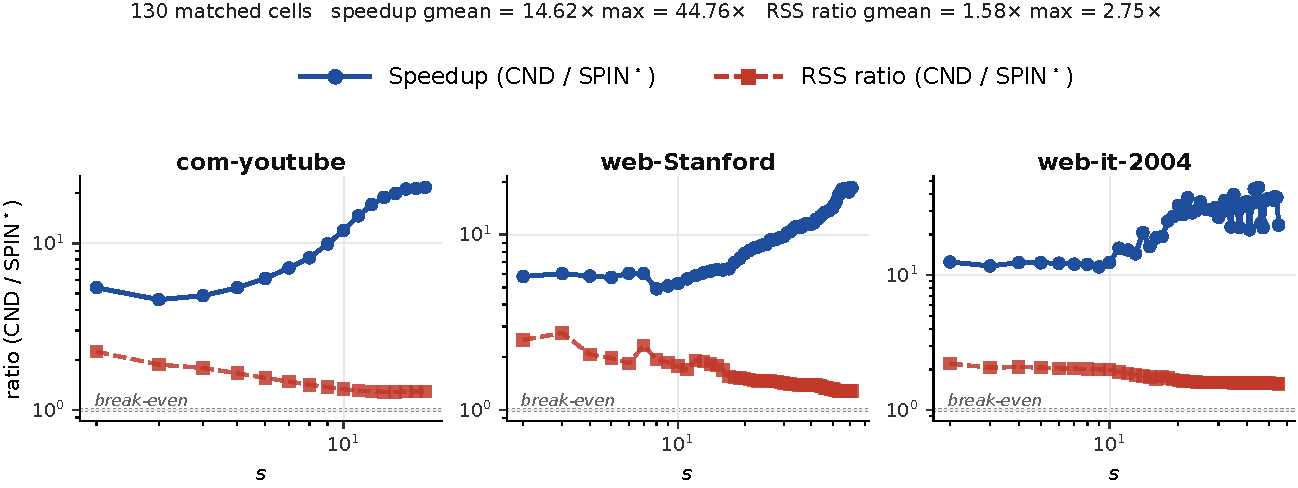
\includegraphics[width=\linewidth]{figures/fig_exp_endtoend.pdf}
\caption{End-to-end comparison on \texttt{com-youtube}, \texttt{web-Stanford}, and \texttt{web-it-2004}.
%
The curves compare the static pipeline with REF on matched successful configurations.
%
Observe that the static pipeline is faster than REF on the matched cells while keeping peak RSS below REF on the plotted ratios.}
\Description{Three-panel plot comparing speedup and memory ratio between the static pipeline and the mutable baseline on the matched subset.}
\label{fig:exp-endtoend}
\end{figure*}

The ten-graph figures show the same qualitative pattern over the broader benchmark suite.
%
Ours is below the REF curve on the plotted time and memory axes.
%
% TODO: verify the ten-graph aggregate against the benchmark source before restoring an aggregate headline.

\begin{figure*}[t]
\centering
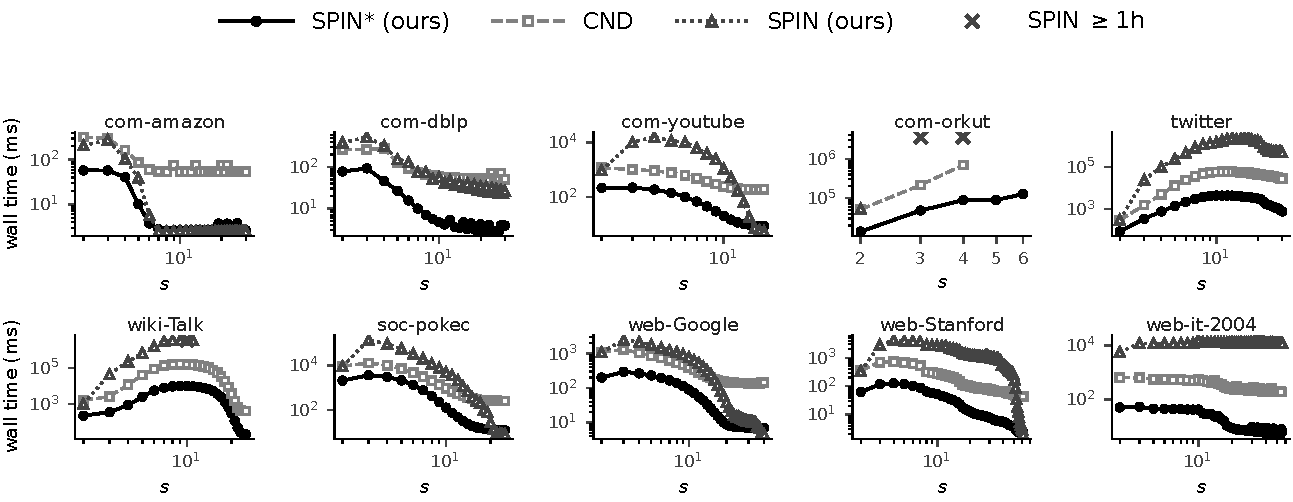
\includegraphics[width=\linewidth]{figures/fig_exp_time.pdf}
\caption{End-to-end wall-clock time as a function of \(s\) in the ten-graph comparison.
%
Solid blue is V3 \peelH{}, and dashed red is the mutable-\cpi{} REF baseline of~\cite{NuclearCD}.
%
Observe how often the blue curve stays below the red curve as \(s\) changes across graph families.
%
The plot shows how the time gap changes with graph family and clique size.}
\Description{A grid of log-scale runtime plots over parameter s, with one subplot per benchmark graph.}
\label{fig:exp-time}
\end{figure*}

\begin{figure*}[t]
\centering
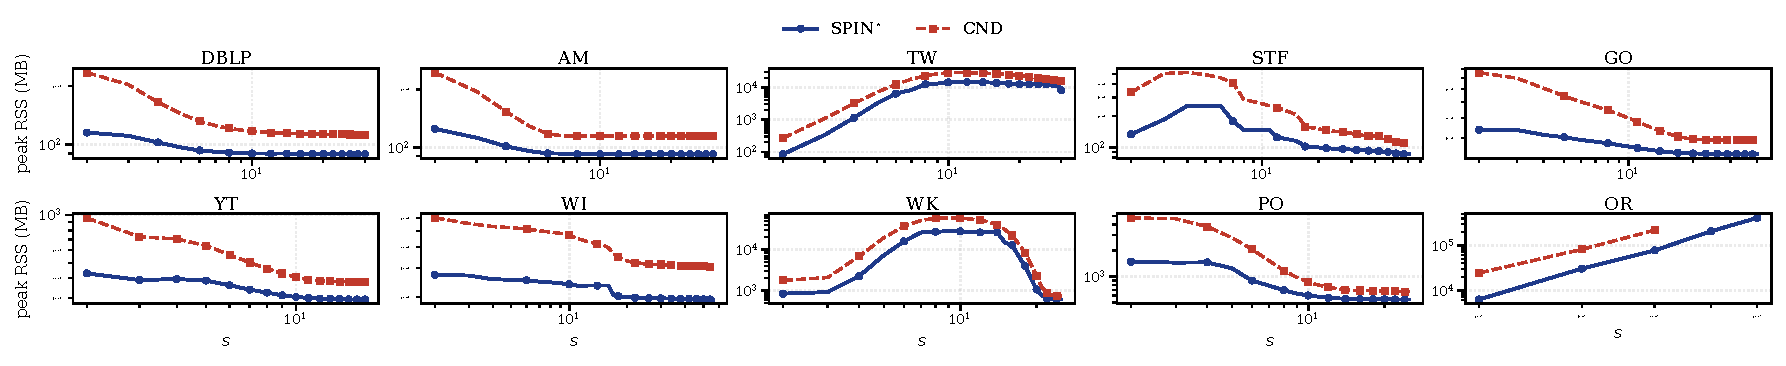
\includegraphics[width=\linewidth]{figures/fig_exp_mem.pdf}
\caption{Peak resident-set memory in the ten-graph comparison.
%
Solid blue is V3, and dashed red is REF.
%
Observe whether flat static incidence storage reduces peak RSS compared with mutable residual \cpi{} state.}
\Description{A grid of log-scale peak-memory plots over parameter s, with one subplot per benchmark graph.}
\label{fig:exp-mem}
\end{figure*}

The memory improvement is explained by the incidence-level budget in Table~\ref{tab:mem}.
%
The mutable baseline stores path hash sets and reverse hash maps.
%
The static pipeline stores flat path-to-vertex and vertex-to-path arrays plus path counters.
%
The analytical per-incidence gap is larger than the observed RSS gap because graph adjacency, allocator overhead, and per-vertex structures do not scale with \(\Sig\).

\begin{table}[t]
\centering
\caption{Memory budget per vertex--path incidence at \(\Sig\gg n\).
%
Baseline numbers are from the mutable-\cpi{} implementation~\cite{NuclearCD}.
%
Our numbers are sizeof-based accounting for the static layout.}
\label{tab:mem}
\small
\begin{tabular}{lrr}
\toprule
\textbf{Component} & \textbf{Baseline} & \textbf{Ours} \\
\midrule
BK recursion tree \(\mathsf{T}\) & \(8\Sig\) & \(0\) \\
Path-to-vertex storage \((V_h,V_p)\) & \(0\) & \(4\Sig\) \\
Per-path vertex set \(\mathsf{H}_P\) & \(32\Sig\) & --- \\
Reverse vertex-to-path map & \(48\Sig\) & --- \\
Vertex-to-path incidence & --- & \(4\Sig\) \\
Support array & \(4n\) & \(4n\) \\
Heap / bucket array & \(24n\) & \(16n+8\kmax\) \\
\midrule
\textbf{Dominant total} & \(\approx 88\Sig\) & \(\approx 10\Sig\) \\
\bottomrule
\end{tabular}
\end{table}

\stitle{RQ3: phase attribution and ablation.}
The phase breakdown explains why the paper optimizes both peeling and construction.
%
After counter-only peeling, construction and loading often dominate total time.
%
On low-\(s\) cases, the peel can still be a visible component.
%
Table~\ref{tab:bd-time} reports representative phase medians.
%
Table~\ref{tab:bd-mem} reports the corresponding memory medians.
%
% TODO: verify the phase subset size and omitted cells against the breakdown source.

\begin{table}[t]
\centering
\caption{Per-phase wall-clock time in ms, median over three runs.}
\label{tab:bd-time}
\scriptsize
\begin{tabular}{llrrrrrr}
\toprule
\multirow{2}{*}{Graph} & \multirow{2}{*}{\(s\)} & \multicolumn{3}{c}{V3} & \multicolumn{3}{c}{REF} \\
\cmidrule(l){3-5}\cmidrule(l){6-8}
& & load & build & peel & load & build & peel \\
\midrule
\texttt{com-youtube}  & 3  & 2081 & 3863 & 440.1 & 1812 & 3982 & 789.7 \\
\texttt{com-youtube}  & 5  & 2028 & 3730 & 273.5 & 1732 & 3795 & 581.6 \\
\texttt{com-youtube}  & 8  & 1967 & 2991 & 86.3  & 1638 & 3053 & 270.2 \\
\texttt{com-youtube}  & 12 & 1689 & 2701 & 13.0  & 1640 & 2649 & 148.5 \\
\texttt{com-youtube}  & 16 & 1640 & 2458 & 8.2   & 1964 & 2488 & 131.8 \\
\midrule
\texttt{web-Stanford} & 3  & 1251 & 6602 & 381.6 & 1250 & 6548 & 521.5 \\
\texttt{web-Stanford} & 10 & 975  & 5840 & 130.4 & 1225 & 5961 & 210.1 \\
\texttt{web-Stanford} & 20 & 999  & 5482 & 28.9  & 1228 & 5591 & 77.8 \\
\texttt{web-Stanford} & 40 & 1224 & 5087 & 9.6   & 1034 & 5007 & 49.6 \\
\texttt{web-Stanford} & 60 & 1224 & 4900 & 1.4   & 1224 & 4907 & 31.3 \\
\midrule
\texttt{web-it-2004}  & 3   & 3389 & 124074 & 351.0 & 3378 & 125347 & 465.9 \\
\texttt{web-it-2004}  & 30  & 3372 & 122558 & 63.9  & 3037 & 122689 & 173.7 \\
\texttt{web-it-2004}  & 100 & 3407 & 121891 & 40.1  & 3377 & 121372 & 135.9 \\
\texttt{web-it-2004}  & 200 & 3416 & 113825 & 26.1  & 3406 & 107516 & 108.5 \\
\texttt{web-it-2004}  & 400 & 3409 & 7850   & 4.6   & 3368 & 7847   & 62.7 \\
\bottomrule
\end{tabular}
\end{table}

\begin{table}[t]
\centering
\caption{Peak resident-set memory in MB, median over three runs.}
\label{tab:bd-mem}
\small
\begin{tabular}{llrrr}
\toprule
Graph & \(s\) & V3 & REF & Ratio \\
\midrule
\texttt{com-youtube}  & 3  & 381 & 729 & \(1.91\times\) \\
\texttt{com-youtube}  & 5  & 315 & 642 & \(2.04\times\) \\
\texttt{com-youtube}  & 8  & 187 & 460 & \(2.45\times\) \\
\texttt{com-youtube}  & 12 & 119 & 385 & \(3.25\times\) \\
\texttt{com-youtube}  & 16 & 114 & 380 & \(3.33\times\) \\
\midrule
\texttt{web-Stanford} & 10 & 176 & 261 & \(1.48\times\) \\
\texttt{web-Stanford} & 40 & 70  & 129 & \(1.85\times\) \\
\texttt{web-Stanford} & 60 & 53  & 111 & \(2.09\times\) \\
\midrule
\texttt{web-it-2004}  & 3   & 425 & 556 & \(1.31\times\) \\
\texttt{web-it-2004}  & 100 & 207 & 296 & \(1.43\times\) \\
\texttt{web-it-2004}  & 400 & 139 & 227 & \(1.63\times\) \\
\bottomrule
\end{tabular}
\end{table}

The ablation separates the state changes.
%
ST isolates the static-incidence state.
%
V2 removes the persistent recursion tree.
%
V3 adds event-driven \peelH{}.
%
% TODO: verify the ablation counts, missing V2 cells, and 3.08x statistic before restoring the ablation headline.

\stitle{RQ4: parallel construction.}
\paraBuild{} exposes seed-level parallelism.
%
Table~\ref{tab:par} reports build time as the thread count grows from \(1\) to \(24\).
%
The table shows strong scaling on web graphs and weaker scaling on smaller or overhead-dominated cases.
%
The correct interpretation is not that construction is perfectly parallel.
%
It is that static output lets the expensive seed walks run without hot-path synchronization.

\begin{table}[t]
\centering
\caption{\paraBuild{} build time in ms, median over three runs.
%
Speedup is \(T=1\) time divided by \(T=24\) time.}
\label{tab:par}
\tiny
\setlength{\tabcolsep}{2pt}
\begin{tabular}{@{}llrrrrrrr@{}}
\toprule
Graph & \(s\) & \(T=1\) & \(T=2\) & \(T=4\) & \(T=8\) & \(T=16\) & \(T=24\) & sp. \\
\midrule
\texttt{com-dblp}      & 3   & 261   & 144   & 90    & 67    & 56   & 54   & \(4.8\times\) \\
\texttt{com-dblp}      & 15  & 232   & 122   & 79    & 57    & 48   & 47   & \(4.9\times\) \\
\texttt{dblp-core30}   & 3   & 47    & 40    & 26    & 20    & 13   & 11   & \(4.3\times\) \\
\texttt{com-youtube}   & 3   & 2719  & 1557  & 835   & 489   & 322  & 464  & \(5.9\times\) \\
\texttt{com-youtube}   & 16  & 2465  & 1384  & 778   & 420   & 258  & 214  & \(11.5\times\) \\
\texttt{web-Stanford}  & 3   & 5470  & 2738  & 1468  & 882   & 477  & 335  & \(16.3\times\) \\
\texttt{web-Stanford}  & 60  & 5296  & 2617  & 1393  & 785   & 424  & 304  & \(17.4\times\) \\
\texttt{web-it-2004}   & 3   & 90432 & 45412 & 23024 & 11908 & 6051 & 4110 & \(22.0\times\) \\
\texttt{web-it-2004}   & 400 & 90275 & 45349 & 22699 & 11692 & 6032 & 3964 & \(22.8\times\) \\
\bottomrule
\end{tabular}
\end{table}

\stitle{RQ5: LocalH behavior.}
\localH{} is the direct fixed-point formulation.
%
It is important because it checks that \peelH{} solves the same equations.
%
LocalH is not intended as the fastest single-machine algorithm.
%
For example, on \texttt{com-dblp} at \(s=10\), sequential V3 finishes the peel in \(7\) ms, while LOCAL\_V4 takes \(396\) s on one thread.
%
The correct conclusion is semantic rather than performance-based: LocalH validates the fixed-point view, while PeelH is the practical realization in this pipeline.
% TODO: verify LOCAL_V4 timings and scaling against raw LocalH experiment logs.

\stitle{RQ6: dense synthetic stress.}
The benchmark graphs are sparse.
%
The stress test follows the dense synthetic protocol used in prior nucleus-decomposition studies~\cite{nucleusSariyuceTODS,NuclearCD}.
%
It generates \(1000\)-vertex graphs by incremental clique injection and sweeps density until the implementations hit the time or memory budget.
%
Both methods grow quickly as density and \(s\) increase.
%
Where both implementations finish, the existing figures show V3 below REF in time and memory.
%
% TODO: verify the stress-test exact density range and reported GB values before restoring the 145GB versus 52GB sentence.

\begin{figure}[t]
\centering
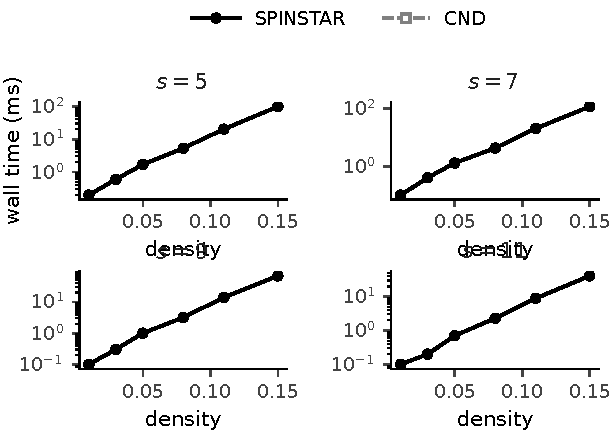
\includegraphics[width=\linewidth]{figures/fig_stress_time.pdf}
\caption{Runtime stress test on synthetic clique-injection graphs with \(|V|=1000\).
%
Solid blue is V3, and dashed red is REF.
%
Observe how quickly runtime grows as density and \(s\) increase.}
\Description{Runtime plots for synthetic dense graphs across several clique sizes and densities.}
\label{fig:stress-time}
\end{figure}

\begin{figure}[t]
\centering
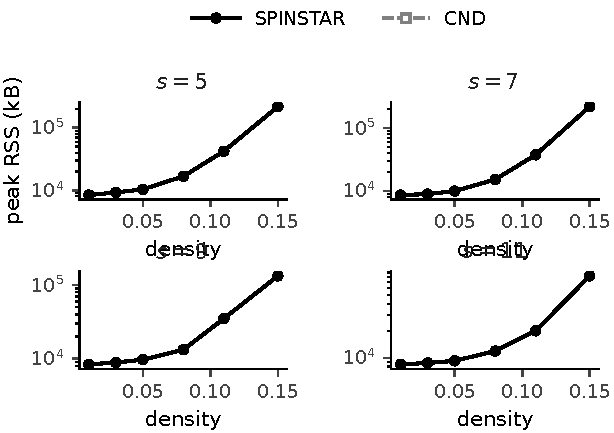
\includegraphics[width=\linewidth]{figures/fig_stress_mem.pdf}
\caption{Peak resident-set memory under the same stress-test protocol as Figure~\ref{fig:stress-time}.
%
Observe whether mutable residual state amplifies memory growth on dense clique-injection instances.}
\Description{Peak-memory plots for synthetic dense graphs across several clique sizes and densities.}
\label{fig:stress-mem}
\end{figure}

% TODO: restore the per-graph ten-graph summary table after verifying every row against the benchmark source.

\stitle{Takeaway.}
The measured facts support two conclusions.
%
First, the static pipeline is faster and uses less peak memory than REF on the \(505\) matched successful configurations in Figure~\ref{fig:exp-endtoend}.
%
Second, the phase and construction experiments show why the optimization chain does not stop at peeling.
